\documentclass[runningheads]{llncs}
%
% PACKAGES AND PATHS
\usepackage{graphicx}
\usepackage{nomencl}
\usepackage{fontawesome}
\usepackage[table]{xcolor} 
\usepackage{xcolor}
\usepackage{float}
\usepackage{wrapfig}
\usepackage{lipsum}
\usepackage{pifont}
\usepackage{array}
\usepackage{url}
\usepackage{subfig}
\graphicspath{ {./imagens/} }
\makenomenclature

%new commands and options
\renewcommand{\topfraction}{.8}
\renewcommand{\arraystretch}{}
\setlength{\abovedisplayskip}{0pt} 


%---------------------------------------------
%BEGIN DOCUMENT
\begin{document}
%
\title{Optimisation of phenylethanol production in \emph{Saccharomyces cerevisiae} and \emph{Escherichia coli}}
%
\author{Rui Gomes\inst{1} \and
Vitor Pereira\inst{2}}

%
\authorrunning{R. Gomes \emph{et al}.}
\titlerunning{Optimization of 2-PE production in \emph{S. cerevisiae} and \emph{E. coli}}
%
\institute{\inst{1}Informatic Department, University of Minho, 4710-057 Braga, Portugal
\email{pg45970@alunos.uminho.pt} \\
\inst{2}Centre of Biological Engineering, University of Minho, 4710-057 Braga, Portugal \\ (Advisor) \\
\email{vpereira@ceb.uminho.pt} \\
\faGithub{ \url{https://github.com/ruigomesbioinf/2-PEopt}} }
%
\maketitle  % typeset the header of the contribution
%
\begin{abstract}
The increasing world demand of resources created an urge in the scientific community to develop and gather better and more suitable tools to fill this gap. As far as biology and computer science are concerned \emph{in silico} approaches can have a great impact in this matter acting like a shortcut to many other unsustainable and non-efficient approaches. Computational strain optimizations together with genome-scale metabolic models open wide doors in this context. In this project strain optimizations using MEWpy were made for trying to increase 2-phenylethanol production in \emph{Saccharomyces cerevisiae} with great success improving this production in almost 4 times the wild-type production as we propose completely new approaches on gene deletions, over expressions and under expressions.

\keywords{MEWpy \and phenylethanol \and  \emph{Saccharomyces cerevisiae} \and \emph{Escherichia coli} \and Genome-scale metabolic model \and Constraints-based models} \and gene over/under-expression \and computational strain optimization

\end{abstract}
%
%
%
\section{Introduction}
\subsection{Context and motivation}
\hspace{0.5cm}The increasing search for sustainable methods and processes that optimize the production of some so-called biological targets created a demand in the scientific community to gather and develop different tools. These tools excel at being sustainable and economical efficient, leaving behind the traditional methods of chemical synthesis and replacing them with biotechnological approaches. Therefore, \emph{in silico} optimization tools have been developed all around the world to provide answers to one of the major challenges of Metabolic Engineering, develop models and algorithms to identify an ensemble of genetic modifications that will translate itself into an optimal strain with the desired phenotype. Most of the time, this means we are searching for the set of modifications that will make the organism have a high yield/production of some target metabolite \cite{rocha2008natural}.

Indeed the optimisation of production of a target metabolite is important and one of the major goals in this matter, however the importance of \emph{in silico} optimisation approaches goes way beyond the maximization of yield/production. Being able to predict via \emph{in silico} approaches, with some margin of error, the set of genetic modification that will result in the optimisation of a given metabolite represents a great amount of costs savings by, for example, deleting sets of modifications that don't correlate with our final objective. This will make sure that the posterior \emph{in vivo} approaches are reduced to a minimal, optimal and predicted working modifications saving millions of dollars in laboratory work \cite{yee2012current}. That's why it's very useful and valuable to use this optimisation tools prior to the laboratory stage. Nevertheless it's also important to remember that these approaches still have some limitations such as their scalability, flexibility and the time needed. The problem of finding optimal gene deletions strategies is combinatorial, which means that the computational time increases exponentially with the size of the problem \cite{rochasilicolife,patil2005evolutionary}.

These set of genetic modifications may be achieved using Linear Programming or optimization meta-heuristics, such as Evolutionary Algorithms (EAs). EAs are population-based stochastic direct search algorithms that in some manner mimic the natural evolution of organisms making the correct assumptions by, as close as possible, simulating this natural environment and natural evolution of things, hence the name Evolutionary Algorithms \cite{bartz2014evolutionary}. EAs follow the next identified set of steps to find the best outcome:
\begin{itemize}
    \item (1) generate offspring by mutating the individuals in the current population;
    \item (2) evaluate the individuals in the population to assert their fitness against one or more optimization objectives,
    \item (3) select the next generation from the offspring and parent population building a new population;
\end{itemize}

All of these is possible due to genome-scale metabolic models (GEMs). They are employed to predict phenotypes resulting from applying an EA solution, a set of genetic modification, and hence allowing to evaluate the fitness of individuals. Since the first GEM of \emph{Haemophilus influenzae} RD was reported in 1999, GEM reconstruction has been one of the most used approaches for system-level metabolic studies \cite{edwards1999systems}. These models represent extensive knowledgebases that provide a platform for model simulations and integrative analysis of omics data. Computationally, a GEM describes a set of stoichiometry-based metabolic reactions of an organism using gene-protein-reaction (GPR) interactions \cite{gu2019current}, enabling metabolic and phenotypic predictions based on some specified constraints. In this project we will be using Yeast8, a \emph{Saccharomyces cerevisiae} genome-scale metabolic model published in 2019 \cite{lu2019consensus} under the Systems and Synthetic Biology group at Chalmers University of Technology, Sweden.

\subsection{Objectives}
\hspace{0.5cm}The main goal of this work is the optimisation of phenylethanol production in \emph{Saccharomyces cerevisiae} and \emph{Escherichia coli}. We will use CSO tools to find the best set of modifications. With this in mind we will: 
\begin{itemize}
    \item[\ding{227}] Revise literature in order to identify strategies used for the maximization of this metabolite in \emph{S. cerevisiae};
    \item[\ding{227}] Conduct \emph{in silico} optimisations using MEWpy \cite{pereira2021mewpy} to find genetic modifications on \emph{S. cerevisiae} that differ from the ones reported in literature;
    \item[\ding{227}] \emph{E. coli} does not naturally produce 2-PE nevertheless, due to some success achieved in reported literature that uses phenylpiruvate as source, we will try the insertion of heterologous reactions and later attempt the optimisation of 2-PE on these \emph{E. coli} engineered strains.
\end{itemize}

\subsection{Methods}

Using the computational resources of the University of Minho "SeARCH Cluster" we will be conducting optimisations under the parameters mentioned in Fig. \ref{fig:methodsscheme}.

\begin{figure}[htbp]
    \centering
    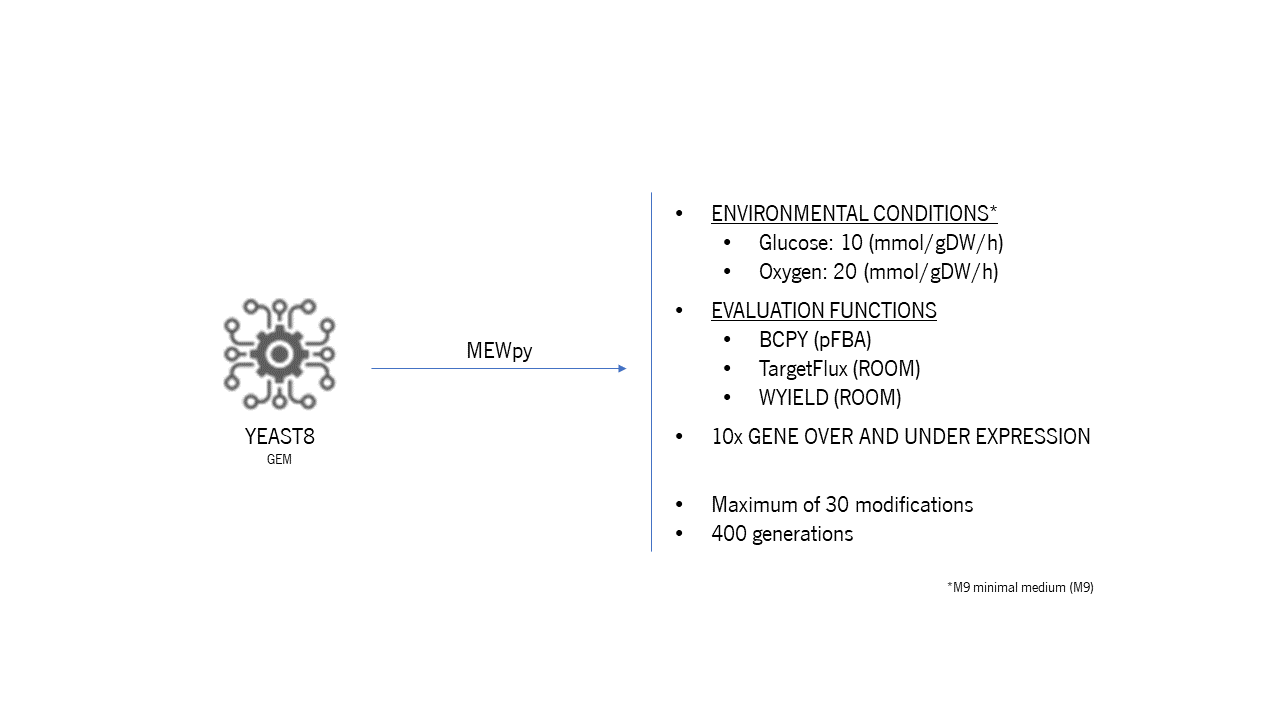
\includegraphics[width=0.60\textwidth]{imagens/METHODS_SCHEME_atualizado.png}
    \caption{Scheme of the main computational objectives of this work including the parameters that will be evaluated during MEWpy optimizations.}
    \label{fig:methodsscheme}
\end{figure}

This optimization setup will be conducted 10 times using the Non-dominated Sorting Genetic Algorithm III (NSGA-III). Once the optimization process ends, solutions will be simplified, removing modifications that do not affect the predicted biomass or product rates.


\section{State of the art}

\subsection{Flux Balance Analysis} 
% Falar em constraint-based modelling|, matriz stoichiométrica| e descrever os métodos de FBA (FBA,pFBA,MOMA,lMOMA,ROOM)
The complete genome for a number of organisms is already available and analysing it is proving itself very useful. The advantages of building mathematical models of cells and simulating their behaviour have long been acknowledged. The power of constraints-based modelling and \emph{in silico} simulations represents a major breakthrough in this field. Useful predictions have been achieved through this \emph{in silico} models such has consequences of gene deletions, optimal growth patterns and shifts in expression profiles. Reportedly, the success rate of this predictions varies from 70\% to 90\% depending on the organism and the type of prediction we're trying to get \cite{price2003genome}.

Constraints-based modelling (CBM) aims to reduce the number of possible fluxes and identify one that most likely will predict the metabolic phenotype of the organism under specific environmental conditions, for example. To test and make these predictions a mathematical structure is given to these models within a matrix S.

Based on a network of biochemical reactions, a stoichiometric matrix S (\(m \cdot n\)) is created, with columns (n) constituting reactions, rows (m) being metabolites, and records S(i, j) representing the stoichiometric coefficient of metabolite i in reaction j. There is a negative coefficient for every metabolite consumed and a positive one for every metabolite produced. A coefficient of zero is used when that metabolite is not used in the reaction. In a large-scale metabolic model there are more reactions than metabolites (n \textgreater m) which means that this will translate in an under-determined system. To solve it additional constraints are
imposed \cite{haggart2011whole}. 

The main assumption imposed on a CBM is the assumption of an internal steady state. This means that we assume that the internal concentration of metabolites do not change over time and we define that as:
\begin{equation} \label{eq:1}
    S \cdot v = 0
\end{equation}
(where \(S\) is the stoichiometric matrix and \(v\) is the matrix of the fluxes).

\begin{figure}[H]
    \centering
    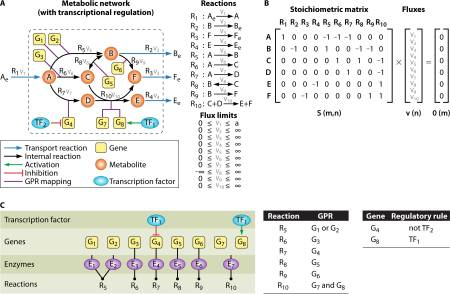
\includegraphics[width=0.60\textwidth]{imagens/stoichiometric_matrix.jpg}
    \caption{A scheme of all the components commonly found in a constraint-based metabolic genome-scale models. (A) Sample network with 10 reactions, 8 genes, 6 metabolites and 2 transcription factors; (B) the corresponding stoichiometric matrix; (C) gene-protein-reaction and transcriptional regulation rules. \cite{maia2016silico}}
    \label{fig:cbmexample}
\end{figure}



There are a variety of phenotype prediction methods with different objectives and analysis. One of the most common approaches for CBM is the use of Flux Balance Analysis (\textbf{FBA}). FBA finds the fluxes of metabolites through metabolic networks and uses linear optimization to predict the steady-state reaction flux distribution in a metabolic network by maximizing an objective function (\emph{i.e.} ATP production or growth rate) \cite{kauffman2003advances,orth2010flux}.

On the same wave, Parsimonious Flux Balance Analysis (\textbf{pFBA}) seeks to minimize the flux associated with each reaction in the model while maintaining optimum flux through the objective function. This method finds the least biologically “expensive” usage of the metabolism of an organism to reach higher growth rates \cite{jenior2020transcriptome}.

Another approach is Minimization Of Metabolic Adjustment (\textbf{MOMA}) and his linear implementation \textbf{lMOMA}. In contrast to FBA, MOMA does not assume optimality of growth or of any other metabolic function. This method was introduced to better understand flux states of mutants and for the prediction of flux distributions in gene knockouts. In essence, MOMA assumes that fluxes in a perturbed cell (mutant) will be redistributed in order to be as close as possible to the wild-type \cite{segre2002analysis}. 

Last but not least, we have Regulatory On/Off Minimization (\textbf{ROOM}). This method represents an constraint-based algorithm that predicts the metabolic steady state of the organism after gene knockouts \cite{shlomi2005regulatory}.


\subsection{Computational Strain Optimization}
% Uma pequena secção sobre computational strain optimization
Computational Strain Optimization (CSO) lays on a metabolic engineering challenge of finding a set of genetic modifications, through \emph{in silico} approaches. These modifications will end up being introduced to an organism. Most of the times they aim to maximize the production of a certain compound of interest while keeping the organism viable.

To achieve this, Computational Strain Optimization Methods (CSOMs) can be acknowledged has procedures used to answer biological questions like "What set of perturbations applied in an organism will favor a desired engineering goal?". There are three main CSOMs:

\textbf{Gene deletion.} To accomplish this task \emph{in silico}, a set of constraints are imposed to the model to force the flux of the disabled reactions to zero followed by the evaluation of the effect of that perturbation.

\textbf{Heterologous insertion.} By inserting nonnative genes or reactions into a model we can expand the metabolic capabilities of it and either boost the yields of native compounds or allow the production of entirely new ones. Later on in this project we will try to do some heterologous insertions on \emph{E.coli} for the production of 2-PE since it can't produce it naturally.

\textbf{Gene over/under expression.} This approach is really useful when the deletion of a gene represents a fatal outcome but downregulation don't. This task is usually implemented through the imposition of additional constraints on the fluxes forcing them to operate near their maximal or minimal bounds. \cite{maia2016silico}

\subsection{MEWpy}
MEWpy \cite{pereira2021mewpy} is a Metabolic Engineering Workbench written in Python that aims to explore different constraint-based models including metabolic, enzymatic or regulatory constraints and provides the implementation of CSO algorithms. The authors in \cite{pereira2021mewpy} proposed MEWpy to fill the gap of lacking integrative tools to explore the increasing amount of modelling approaches.

\subsubsection{MEWpy Architecture.}
The conceptual structure of this workbench is highlighted in Figure \ref{fig:mewpyarch} and his environment has three essential layers, from bottom to top:

\begin{figure}[H]
    \centering
    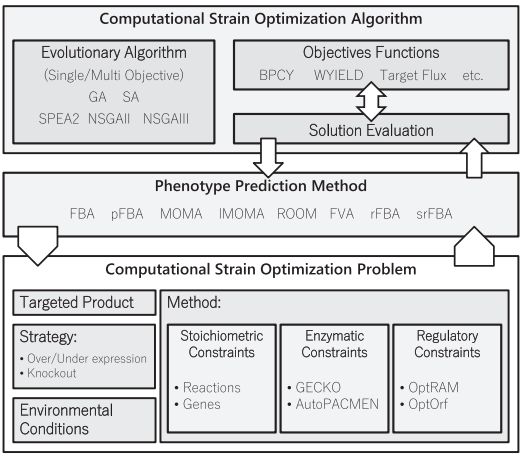
\includegraphics[width=0.50\textwidth]{imagens/mewpy_architecture.png}
    \caption{Conceptual architecture of the MEWpy framework. \cite{pereira2021mewpy}}
    \label{fig:mewpyarch}
\end{figure}

\subsubsection{Objective Functions}
The optimization task relies greatly on the employed objective functions. MEWpy makes available the following:
\begin{itemize}
    \item[\ding{227}] \textbf{Biomass-Product Coupled Yield (BPCY)} \\
    The maximization of Biomass-Product Coupled Yield is considered one of the most used objective functions in CSO.
    \begin{equation}
        BPCY = Product \times Growth
    \end{equation}
    And can also account for a carbon source or substrate consumption:
    \begin{equation}
        BPCY = \frac{Product \times Growth}{Substrate}
    \end{equation}
    \item[\ding{227}] \textbf{Target Flux} \\
    This is the most straight forward objective function. The goal is to maximize the production of a target product.
    \item[\ding{227}] \textbf{Weighed Yield (WYIELD)} \\
    Objective function that embraces the target product flux variability, constrained to a minimal growth and introduced metabolic modifications.
    \begin{equation}
        WYIELD = \alpha \times FVA\textsubscript{max}(Product) + (1 - \alpha) \times FVA\textsubscript{min}(Product)
    \end{equation}
    \item[\ding{227}] \textbf{Modification Type} \\
    This objective favors modifications with deletions and down regulations. As such, a solution that encompasses more deletions is considered better than one with many up regulations.
    \item[\ding{227}] \textbf{Candidate Size} \\
    Problems definition allows for setting a maximum number of modifications.
\end{itemize}

\subsection{2-phenylethanol}
Aromatic compounds often hold a sweet or pleasant aroma and are widely used in the chemical industry \cite{aromaticcoumounds}. 2-PE, discovered in 1876, is a highly aromatic alcohol characterized by a rose-like odour that is greatly used in perfume, cosmetics and even in the food industry being the main commercial alcohol \cite{fabre1998phenylethyl,etschmann2002biotechnological}. By the year 2020 2-PE market size surpassed 240 million USD and the projections indicate that until 2027 the market size can increase 5,5 \% \cite{globalmarketinsightsinc}, hence the importance of optimise the production of this compound.

2-PE can be found naturally in the essential oils of some plants and flowers. However, for the majority of cases, the concentrations are too low to be extracted efficiently. That, along with the costs of extraction being to high to justify it and the increasing demand of consumers and industry for this compound, makes it unsustainable to be naturally produced. That's why the vast majority of this compound is produced via biochemical approaches \cite{etschmann2002biotechnological}.

With this in mind there are a collection of yeasts that are able to produce 2-PE naturally which includes \emph{Saccharomyces cerevisiae}, \emph{Kluyveromyces
marxianus}, \emph{Kluyveromyces lactis}, \emph{Pichia fermentans}, \emph{Pichia anomala},
\emph{Schizosaccharomyces pombe}, and \emph{Hansenula anomala} \cite{etschmann2003screening} and they do that via two main routes, the Ehrlich pathway and the Shikimate pathway.

\textbf{Ehrlich pathway}

First described by Ehrlich, hence the name, in 1907 \cite{EhrlichberDB}, this pathway is well characterized for producing 2-PE in the model organism \emph{S. cerevisiae}.
This pathway is rather convenient and fast to synthesize 2-PE mainly because it has only three reaction steps using L-phenylalanine as the substrate. These three reactions consists of a transamination of L-phenylalanine in phenylpyruvate, which is then transformed to phenylacetaldehyde by decarboxylation and finally this phenylacetaldehyde is reduced to 2-PE by dehydrogenation \cite{hazelwood2008ehrlich}. (Figure \ref{fig:metabolicpathways})

\begin{figure}[H]
    \centering
    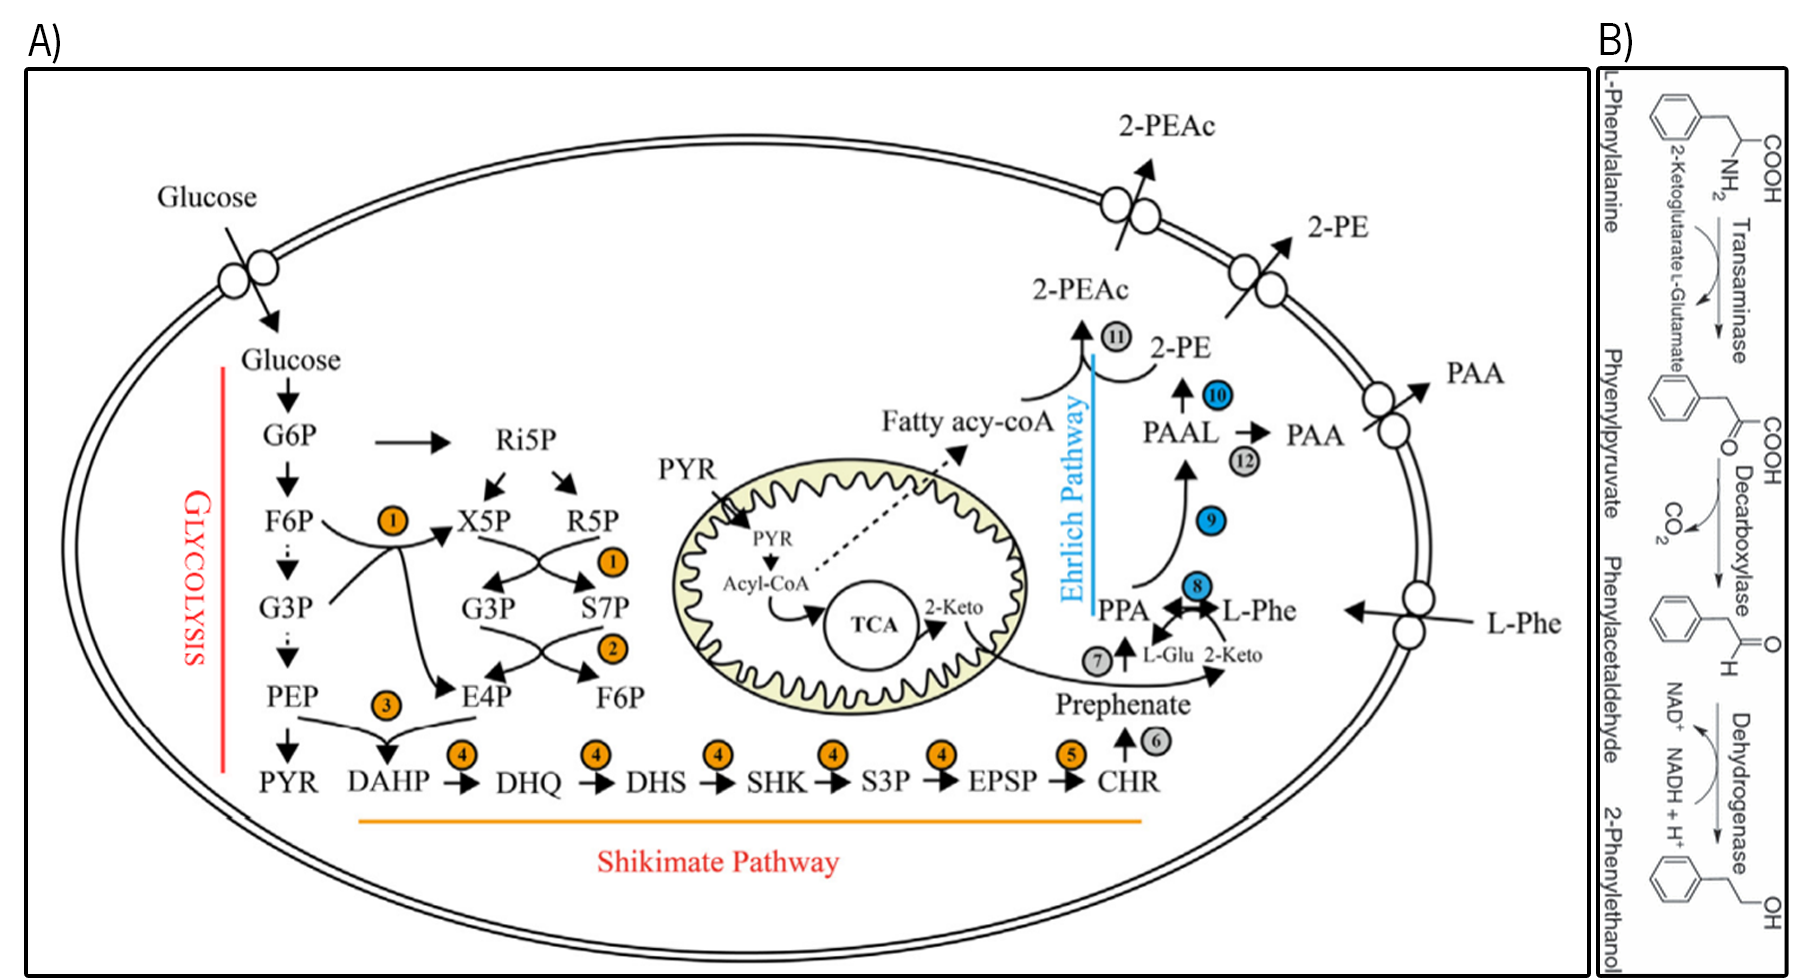
\includegraphics[width=0.75\textwidth]{imagens/DETAILED_PATHWAY.png}
    \caption{A) Metabolic pathways for 2-PE production in Yeasts. Ehrlich pathway (blue), Shikimate pathway (yellow), Glycolysis (red). Adapted from \cite{wang2019advances}; B) Detailed Ehrlich pathway for 2-PE synthesis \cite{etschmann2002biotechnological}}
    \label{fig:metabolicpathways}
\end{figure}

\textbf{Shikimate pathway}

This pathway synthesizes 2-PE de novo from glucose, although the efficiency is quite low due to feedback regulations in many branched metabolic pathways \cite{yin2015improving}, via the phenylpyruvate pathway, which is a combination of the Shikimate and Erhlich pathways. In this pathway, phosphoenolpyruvate (PEP) and erythrose 4-phosphate (E4P) are combined to synthesize 3-deoxy-d-arabino-heptulosonate-7-phosphate (DAHP), which is then converted to phenylpyruvate (PPA) in several other metabolic steps (Figure \ref{fig:metabolicpathways}). Phenylpyruvate will then be converted to 2-P2 by decarboxylation and dehydrogenation as described previously in the Erhlich pathway. \\

\textbf{Approaches to improve 2-PE production in \emph{S. cerevisiae}}

A lot has been done to improve the production of 2-PE through biotechnological approaches via the Ehrlich pathway and the Shikimate pathway. With the Ehrlich pathway being the main route for the production of this compound studies were made in order to understand these organism-pathway interactions. In this pathway, the flux from L-Phe towards phenylacetaldehyde represents the main limitation factor for a higher titer of 2-PE, thus increasing the activity of aminotransferase or decarboxylase has been applied in order to improve 2-PE accumulation, so in some studies both aromatic aminotransferase I \emph{ARO8} and aromatic aminotransferase II \emph{ARO9} have been over expressed resulting in varying proportions of improvement of our coumpound titer \cite{kim2014metabolic,yin2015improving}. The decarboxylation reaction of this pathway has five likely genes capable of encoding decarboxylases but studies proved that \emph{ARO10} was more than sufficient to encode phenylpyruvate decarboxylase even when the other four genes were inactivated \cite{yin2015improving,wang2019advances}. Therefore, the over expression of aromatic aminotransferase I \emph{ARO8} and phenylpyruvate descarboxylase \emph{ARO10}, that catalyzes decarboxylation of phenylpyruvate to phenylacetaldehyde, produced an increase of 2-PE production between 36.8\% and 218\% when compared to a parental strain. This study also refers that to accelerate the L-Phe transportation rate in \emph{S. cerevisiae} some studies improved the expression levels of \emph{GAP1} gene, responsible for an amino acid permease, which led to an 25.3\% increase of 2-PE \cite{qian2019current,wang2019advances}. Phenylacetaldehyde is competitively converted to phenylacetic acid by aldehyde dehydrogenase and the deletion of both \emph{ALD2} and \emph{ALD3} (cytoplasmic aldehyde dehydrogenases) resulted in 30\% of 2-PE titer. On the other hand, over expression of alcohol dehydrogenase \emph{ADH} genes produced no effect on 2-PE production. over expressing \emph{GAP1} led to an increase of the intracellular level of L-Phe which led to an increase of 79\% of 2-PE titer. over expressing glutamate dehydrogenase gene \emph{GDH2} improved the regeneration of NAD(P)H which resulted in an improved titer of 2-PE. \cite{wang2019advances} 

\textbf{\emph{E.coli} heterologous reactions introduction}

For the main \emph{E.coli} chassis we used the iML1515 model for this organism, available at BiGG Models database \cite{biggmodels}. By the time we first used it this model already had the Glycolisys and the Shikimate pathway, however it did not had the main key for the production of 2-PE, the Erhlich pathway. With that said we introduced the Ehrlich pathway (a total of 3 reactions) to the said model using COBRApy \cite{cobrapy}. By this time it was also necessary to add 2-PE as a metabolite because this organism, as we have mentioned, doesn´t naturally produce it.

\section{Results}
After all the optimizations were run in the SeARCH University of Minho Cluster services, the outputs of all 10 optimizations were processed using a set of python libraries that turned out to be very helpful in the process, some examples are: pandas, glob and ast.
All these solutions retrieved by MEWpy passed four main filtering methods. From the pool of all possible solutions we've selected the ones that:
\begin{itemize}
    \item[\ding{227}] Had a biomass higher than 0.1, important to make sure that our organism stays biologically viable;
    \item[\ding{227}] Accounted for a maximum of 15 gene modifications;
    \item[\ding{227}] Were defined by having more gene knockouts and/or down-regulations rather than up-regulations;
    \item[\ding{227}] Had a minimum FVA value higher than 0;
\end{itemize}

The values of biomass used to filter our initial dataframe were obtained by following the next equation: \[ Biomass = \frac{BPCY}{phenylethanol flux} \]



A maximum of 15 modifications were taken into account and this value was chosen arbitrarily in order to narrow down our possible set of solutions.
Our decision of selecting solutions that had more gene knockouts and/or down-regulations in opposition to up-regulations was mainly because it's easier to implement knockouts and down-regulations at wet lab conditions than up-regulations. However we cannot fully discard these solutions because in certain conditions it can be valuable to implement more up-regulations, depending on the final flux of our target. The same goes with the biomass values, the higher the biomass value the quickest our organism multiplies itself and consequently the aggregated production of our target increases.

With that being said, we started our data preprocessing stage with a total of 189 possible solutions that comprised the modification of expression of a total of 318 genes in a range of 1 to 24 gene expression modifications, per solution. We managed to scale it down to 5 reasonable solutions accounting for a total of 15 genes. These solutions can be consulted in Table \ref{tab:final_solutions} of this project, available in the appendices at the end of this document.

Of all 5 modifications, we will treat the highlighted ones as case studies. We will analyse in-depth the first one mainly because it's the one that gives us the higher 2-phenylethanol flux rate. The second highlighted one will be analysed in-depth due to the fact that it is the one that best correlates with our criteria of having more knockouts and down-regulations than up-regulations.

\subsection{Case studies}
The first solution that we will look over consists of 4 gene over expressions and 4 gene under expressions. As far as over expressions are concerned this solution tells us to over express YGR256W, YCL050C, YNL316C and YPR145W genes. The YGR256W represents a gene that encodes 6-phosphogluconate dehydrogenase (GND2) which is responsible for the biosynthesis of secondary metabolites and it has an active function on the pentose phosphate pathway by catalyzing the oxidative decarboxylation of 6-phosphogluconate to ribulose 5-phosphate. YCL050C encodes a phosphorylase that catalyzes the phosphorolytic degradation of bis(5'-adenosyl) tetraphosphate (Ap4A) into ADP and ATP. YNL316C encodes prephenate dehydratase (PHA2) which catalyse the decarboxylation/dehydration of prephenate to phenylpyruvate, it's also involved in L-phenylalanine biosynthesis. YPR145W encodes a protein (ASN1) involved in aspargine synthesis, converts glutamine and aspartate to glutamato and asparagine. On the other hand, this solution has YDL198C, YLR359W, YDR497C and Q0045 as gene under expression. YDL198C encodes a mitochondrial GTP/GDP carrier protein (GGC1) that's responsible for GTP uptake and GDP exit from mithocondria. YLR359W encodes the ADE13 protein that helps catalyse, in two non-sequential steps, in de novo AMP synthesis. It's also involved in the production of fumarate. YDR497C encodes ITR1 protein, a myo-inositol transporter involved in pseudohyphal growth, a process in which cells grow as a chain physically attached cells in response to a stimulus. Q0045 is the gene that encodes COX1 protein, a protein that is the main component of the cytochrome c oxidase, the last enzyme in the mitochondrial electron transport chain which drives oxidative phosphorylation contributing to the transfer of electrons from cytochrome c to oxygen resulting in the formation of water.

The second highlighted solution appears to be, of all the other, the one that has the most value. Not only it's the one that better corresponds with our selection/filtering criteria but it also represent the highest biomass value of them all and the flux rate value is somewhat close to the highest value in the pool of solutions. This solution accounts for 2 over expressions of YGR256W and YNL316C genes, a under expression of the gene Q0045 and finally 3 gene deletions YDR111C, YGL202W and YJR095W. The genes that represent over and under expressions in this solution were already mentioned and over viewed before. In regard of the gene deletions suggested by this solution we have the deletion of YDR111C that encodes a catalytically inactive alanine transaminase (ALT2) and his expression is repressed in the presence of alanine. Next we have the deletion of YGL202W that encodes an aromatic aminotransferase (ARO8) who was already approached in this study, however some literature already mentioned used an over expression approach rather than a deletion approach. Last but not least we have the deletion of YJR095W, a gene that encodes a mithocondrial succinate-fumarate transporter (SFC1) which transports succinate into and fumarate out of the mithocondrion.

MEWpy makes possible to plot flux envelopes. We plotted the flux envelopes for the two solutions and the results of this can be seen at Fig. \ref{fig:flux_envelopes}.

\begin{figure}[]
  \centering
  \subfloat[Flux envelope of solution 1]{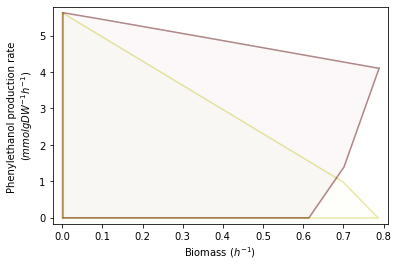
\includegraphics[width=0.4\textwidth]{imagens/solution1.png.jpg}\label{fig:flux_envelope_sol1}}
  \hfill
  \subfloat[Flux envelope of solution 4]{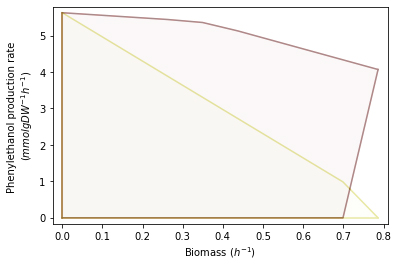
\includegraphics[width=0.4\textwidth]{imagens/solution2.png.jpg}\label{fig:flux_envelope_sol2}}
  \caption{Production flux envelopes of 2-phenylethanol for the solutions analysed compared to the wild-type (yellow envelope) of \emph{Sacharomyces cerevisiae}. With oxygen uptake of 20 $(mol gDW^{-1} h^{-1})$ and glucose uptake of 10 $(mol gDW^{-1} h^{-1})$}
  \label{fig:flux_envelopes}
\end{figure}

The envelope production plots let us see how our model behaves by computing the minimal and maximal 2-phenylethanol production rates at different rates of biomass production. As we can see both these solutions are somewhat capable of increasing the production rate of 2-phenylethanol in \emph{Saccharomyces cerevisiae} with both maximum values being very close to each other. It's important to say that while both approaches can be of some value solution 4 might be the way to go since, as we mentioned before, has less upregulation, making it easier to implement in wet-lab conditions.
\section{Conclusion}
Computational strain optimizations has proven to be a very reliable way of engineer better and most capable organism strains in order to maximize the production of certain targets. It's a high potential process and everyday a huge community is trying to keep improving these methods and algorithms. MEWpy is a great example of this, a powerful metabolic engineering workbench modelled by man, designed by nature as the authors like to say.
With this project we were able to predict the phenotype of \emph{Saccharomyces cerevisiae} by computing a valuable set of gene modifications. We managed to narrow it down to 5, predictably best, solutions but many more could have been ignored due to our selection criteria. However, with this selection steps we believe we have made the right choices in terms of what can be done in real life with this organism considering the reality of things.
Interesting enough is the fact that some modifications within our solutions doesn't correlate with or are even mentioned in any literature reported. This can actually be a good or a bad thing since only a in vivo confirmation could answer this types of questions. A good example of this is the fact that some literature approaches the over expression of an aromatic aminotransferase called ARO8 while MEWpy chooses to make a deletion of that same ARO8. While it makes this dystopian choices it also chooses, for example, to over express the YNL316C gene which encodes an enzyme capable of producing phenylpyruvate (a very important metabolite in the 2-phenylethanol pathway) with prephenate.
In regard of the \emph{E.coli} part of this project a lack of time, no results retrieved and misunderstanding of the problem lead to not having results and therefore no further analysis were made in this context. However, the model with an heterologous Ehrlich pathway was made, edited from the main chassis iML1515 model and it's available at my GitHub repository for this essay.
For the future it can be favorable to try and experiment these solutions in vivo which can also be a way of validate even more MEWpy and his capabilities. It can also be beneficial to implement optimisations on the edited \emph{E.coli} model for further understanding of this matter and to eventually make the best to try and make \emph{E.coli} naturally produce 2-phenylethanol.
\section{Code availability}
Python files used in this project as well as the models and all the complementary material can be found at: \url{https://github.com/ruigomesbioinf/2-PEopt}

\clearpage



% ---- Bibliography ----
%
% BibTeX users should specify bibliography style 'splncs04'.
% References will then be sorted and formatted in the correct style.
%
\bibliographystyle{ieeetr}
\bibliography{mybibliography.bib}

% ---- nomenclature ----
\nomenclature{2-PE}{2-phenylethanol}
\nomenclature{EA}{Evolutionary Algorithm}
\nomenclature{EP}{Evolutionary Programming}
\nomenclature{GEMs}{Genome-scale metabolic models}
\nomenclature{GPR}{Gene-Protein-Reaction}
\nomenclature{L-Phe}{L-Phenilalanine}
\nomenclature{CBM}{Constraints-based model}
\nomenclature{FBA}{Flux Balance Analysis}
\nomenclature{pFBA}{Parsimonious FBA}
\nomenclature{CSO}{Computational Strain Optimization}
\nomenclature{CSOMs}{Computational Strain Optimization Methods}
\nomenclature{MOMA}{Minimization of Metabolic Adjustment}
\nomenclature{lMOMA}{Linear Minimization of Metabolic Adjustment}
\nomenclature{ROOM}{Regulatory On/Off Minimization}
\nomenclature{BPCY}{Biomass-Product Coupled Yield}
\nomenclature{WYIELD}{Weighed Yield}
\printnomenclature

\newpage
% ---- Appendices ----
\section{Appendices}

\begin{table}[H]
    \centering
    \begin{tabular}{||c|c|c|>{\centering\arraybackslash} m{2cm}|c|c||}
    \hline
    BPCY & TargetFlux & WYIELD & Gene & \shortstack{Biomass \\ \[h^{-1}\]} & \shortstack{Flux rate \\ \[(mol gDW^{-1} h^{-1}) \]} \\ [0.5ex] 
    \hline \hline
    0.398820 & 0.102054	& 3.550329 &  \shortstack{\\ YPL028W \otimes \\ YNL316C \uparrow \\ YMR105C \uparrow \\ YHR183W \uparrow \\ YOR065W \downarrow} & 0.429966 & 3.753913 \\
    \hline
    \rowcolor{yellow!30} 0.311934 & 0.077422	& 3.702119 & \shortstack{\\ YGR256W \uparrow \\ YDL198C \downarrow \\ YLR359W \downarrow \\ YCL050C \uparrow \\ YDR497C \downarrow \\ YNL316C \uparrow \\ Q0045 \downarrow \\ YPR145W \uparrow} & 0.336295 & 3.858282 \\
    \hline
    0.311934 & 0.077422	& 3.702119 & \shortstack{\\ YGR256W \uparrow \\ YNL316C \uparrow \\ Q0045 \downarrow} & 0.513125 & 3.851711 \\
    \hline
    0.439335 & 0.110119	& 3.613078 & \shortstack{\\ YGR256W \uparrow \\ YNL316C \uparrow \\ Q0045 \downarrow \\ YDR111C \otimes \\ YGL202W \otimes \\ YPR145W \uparrow} & 0.473645 & 3.835133 \\
    \hline
    \rowcolor{yellow!30} 0.477147 & 0.119819 & 3.588457 & \shortstack{\\ YGR256W \uparrow \\ YNL316C \uparrow \\ Q0045 \downarrow \\ YDR111C \otimes \\ YGL202W \otimes \\ YJR095W \otimes} & 0.514409 & 3.830782 \\ [1ex]
    \hline
    \end{tabular}
    \caption{Table of possible solutions, retrieved by MEWpy, after the preprocessing stage. \uparrow upregulation, \downarrow downregulation, \otimes deletion}
    \label{tab:final_solutions}
\end{table}
\end{document}
